\begin{figure}[htbp]
\centering
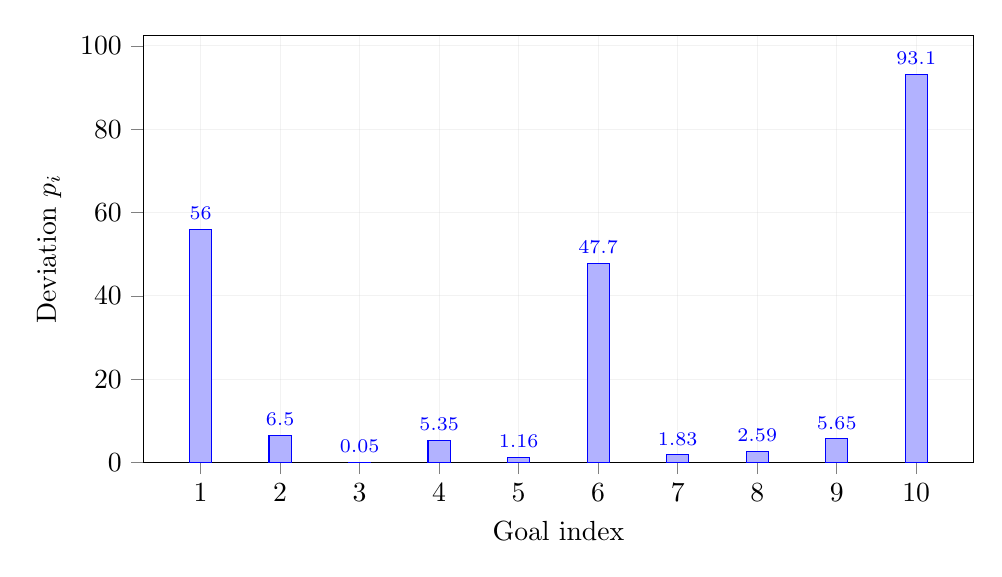
\begin{tikzpicture}
\begin{axis}[
    ybar,
    ymin=0,
    width=\textwidth,
    height=7cm,
    bar width=8pt,
    enlarge x limits=0.08,
    ylabel={Deviation $p_i$},
    xlabel={Goal index},
    xtick=data,
    xticklabel style={/pgf/number format/precision=0},
    nodes near coords,
    nodes near coords align={vertical},
    every node near coord/.append style={font=\scriptsize, /pgf/number format/fixed},
    tick align=outside,
    tick pos=left,
    grid=both,
    grid style={opacity=0.2},
]
\addplot coordinates
{ (1,56.00) (2,6.50) (3,0.05) (4,5.35) (5,1.16)
  (6,47.70) (7,1.83) (8,2.59) (9,5.65) (10,93.10) };
\end{axis}
\end{tikzpicture}
\caption{Weighted Goal Programming — deviations above targets ($p_i$) for each goal.}
\label{fig:wgpDeviationsChart}
\end{figure}
